\documentclass[tikz, margin=5mm]{standalone}

\usepackage{pgfplots}
\pgfplotsset{compat=1.18}
\usetikzlibrary{patterns}

\begin{document}
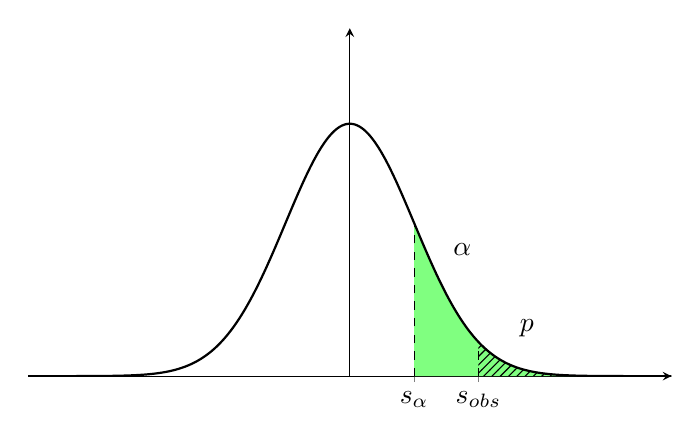
\begin{tikzpicture}
    \begin{axis}[
        xtick={1, 2}, ytick=\empty,
        xticklabels={$s_{\alpha}$, $s_{obs}$},
        axis x line=middle,
        axis y line=middle,
        domain=-5:5, smooth, samples=300,
        ymax=.55,
        width=9.75cm, height=6cm,
    ]
        \addplot[fill=green!50, draw=none, domain=1:5] {1/(1*sqrt(2*pi))*exp(-((x-0)^2)/(2*1^2))} \closedcycle;
        \draw[dashed] (axis cs: 1, 0) -- (axis cs: 1, {1/(1*sqrt(2*pi))*exp(-((1-0)^2)/(2*1^2))});
        \addplot[pattern color=black, pattern = north east lines, draw=none, domain=2:5] {1/(1*sqrt(2*pi))*exp(-((x-0)^2)/(2*1^2))} \closedcycle;
        \draw[dashed] (axis cs: 2, 0) -- (axis cs: 2, {1/(1*sqrt(2*pi))*exp(-((2-0)^2)/(2*1^2))});
        \node at (axis cs: 1.75, 0.2) {$\alpha$};
        \node at (axis cs: 2.75, 0.075) {$p$};
        \addplot[thick, black] {1/(1*sqrt(2*pi))*exp(-((x-0)^2)/(2*1^2))};
    \end{axis}
\end{tikzpicture}
\end{document}